\documentclass{slide}

\usepackage{changepage}
\usepackage{tabto}
% \usepackage{pgfpages}
% \setbeameroption{show notes on second screen}

\title{Serverless Architecture}
\subtitle{Software Architecture}
\author{Richard Thomas}
\date{\week{12}}

\begin{document}

\maketitle

\oxymoron{Serverless}{Logic running on someone else's server.}
\note{Developers can focus on logic, not infrastructure to deliver it.}

\definition{Backend as a Service (BaaS)}{Cloud-hosted applications or services that deliver functionality used by an application front-end.}
\note[itemize]{
    \item Front-end may be a SPA or mobile app.
    \item Back-end provides sophisticated functionality (e.g. database, machine learning, location services, authentication, \dots).
    \item Front-end ties back-end services together to deliver the application's functionality.
}

\begin{frame}{BaaS Iceberg \cite{serverless-images}}
    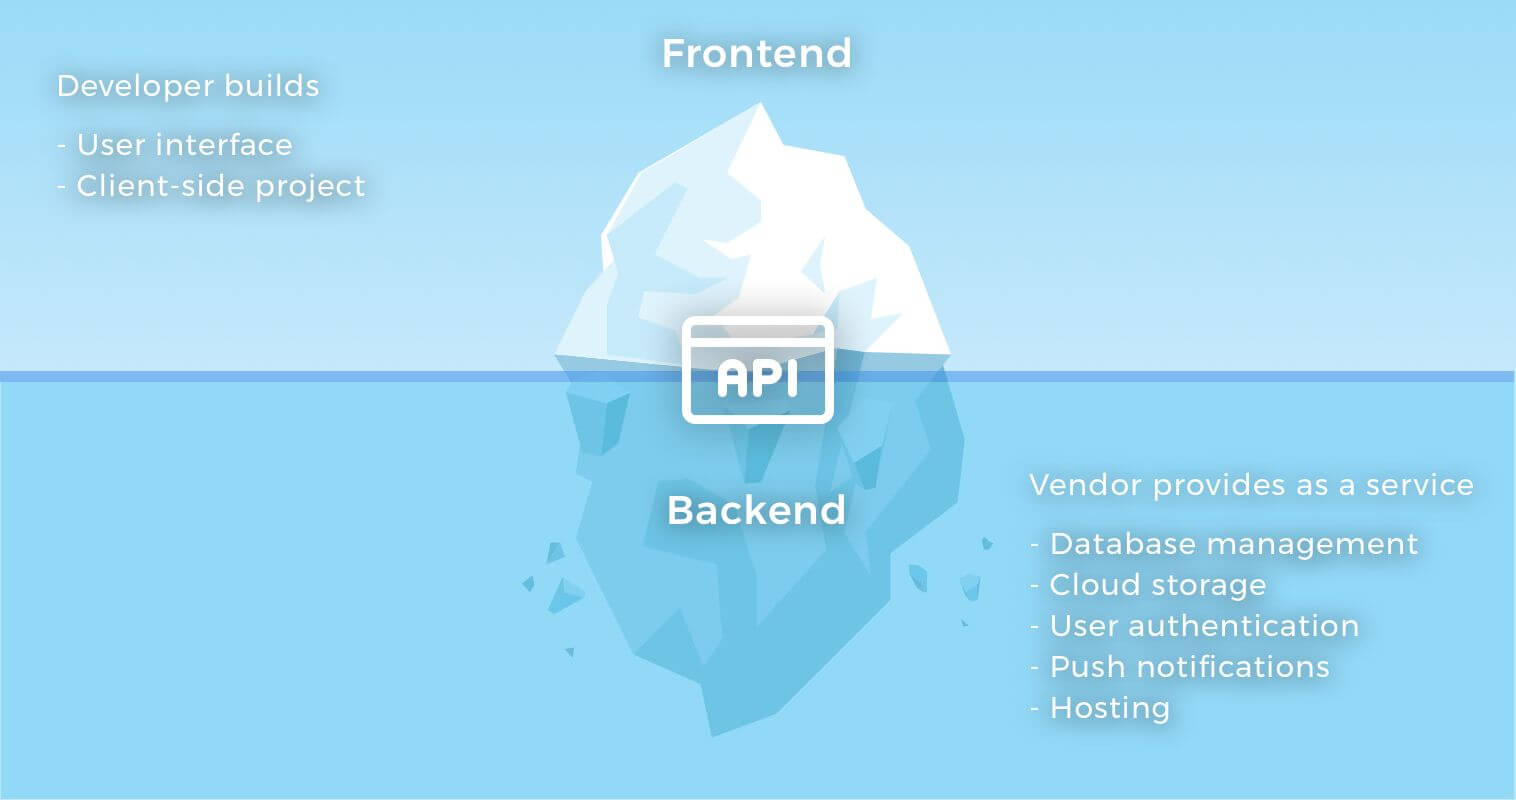
\includegraphics[width=\textwidth]{images/baas.jpg}
\end{frame}

\begin{frame}{BaaS Example}
    \begin{adjustwidth}{-12mm}{-12mm}
        \centering
        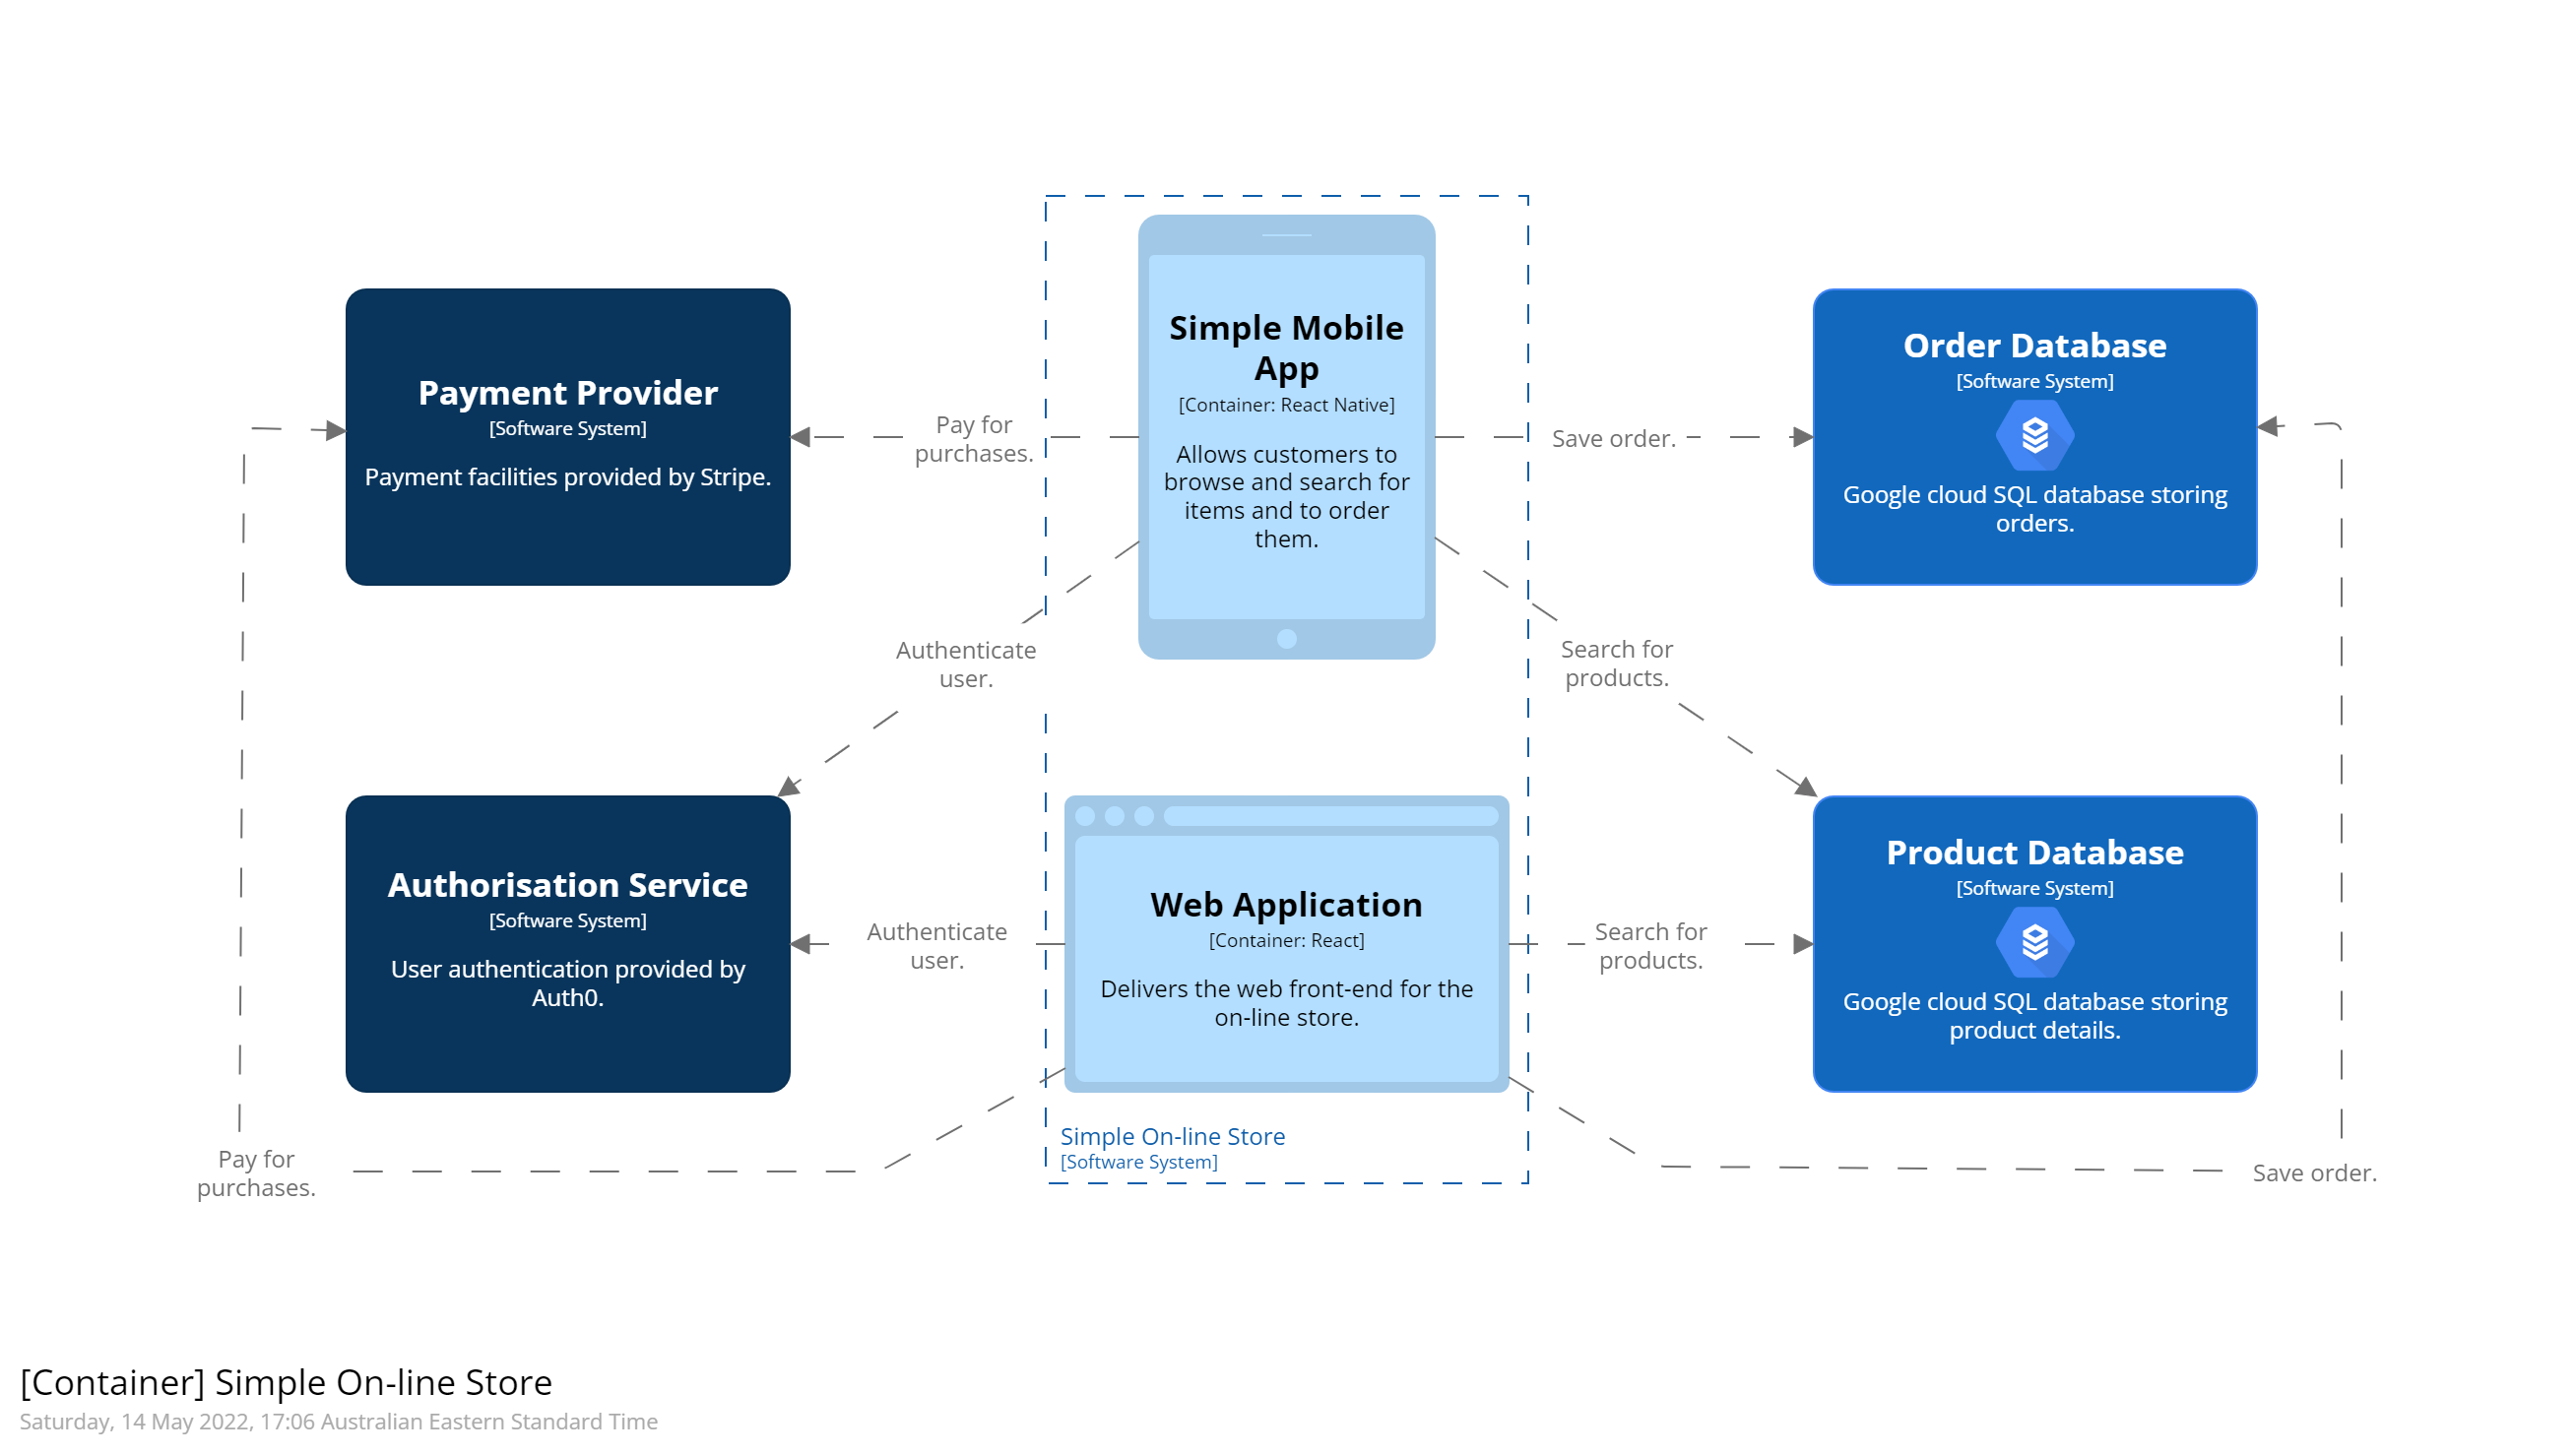
\includegraphics[trim=195 195 195 195,clip,width=0.98\paperwidth]{diagrams/baas-example.png}
    \end{adjustwidth}
\end{frame}
\note[itemize]{
    \item Example of simple system with back-end functionality delivered entirely via BaaS.
    \item Feature-rich front-ends coordinate behaviour delivered by BaaS.
    \item Consequence: Front-ends are tightly coupled to BaaS.
    \item Consequence: Front-ends are have both UI and functional behaviour logic.
    \item Front-end could have a layered design, though many SPAs don't.
}

\definition{Functions as a Service (FaaS)}{Application logic that is triggered by an event and runs in a transient, stateless compute node.}
\note[itemize]{
    \item Node may only exist for duration of function call.
    \item Server infrastructure (e.g. type of node, lifespan, scaling, \dots) are managed by hosting provider.
    \item e.g. AWS Lambda, Google App Engine, Azure Automation, \dots.
}

\begin{frame}{FaaS Iceberg \cite{serverless-images}}
    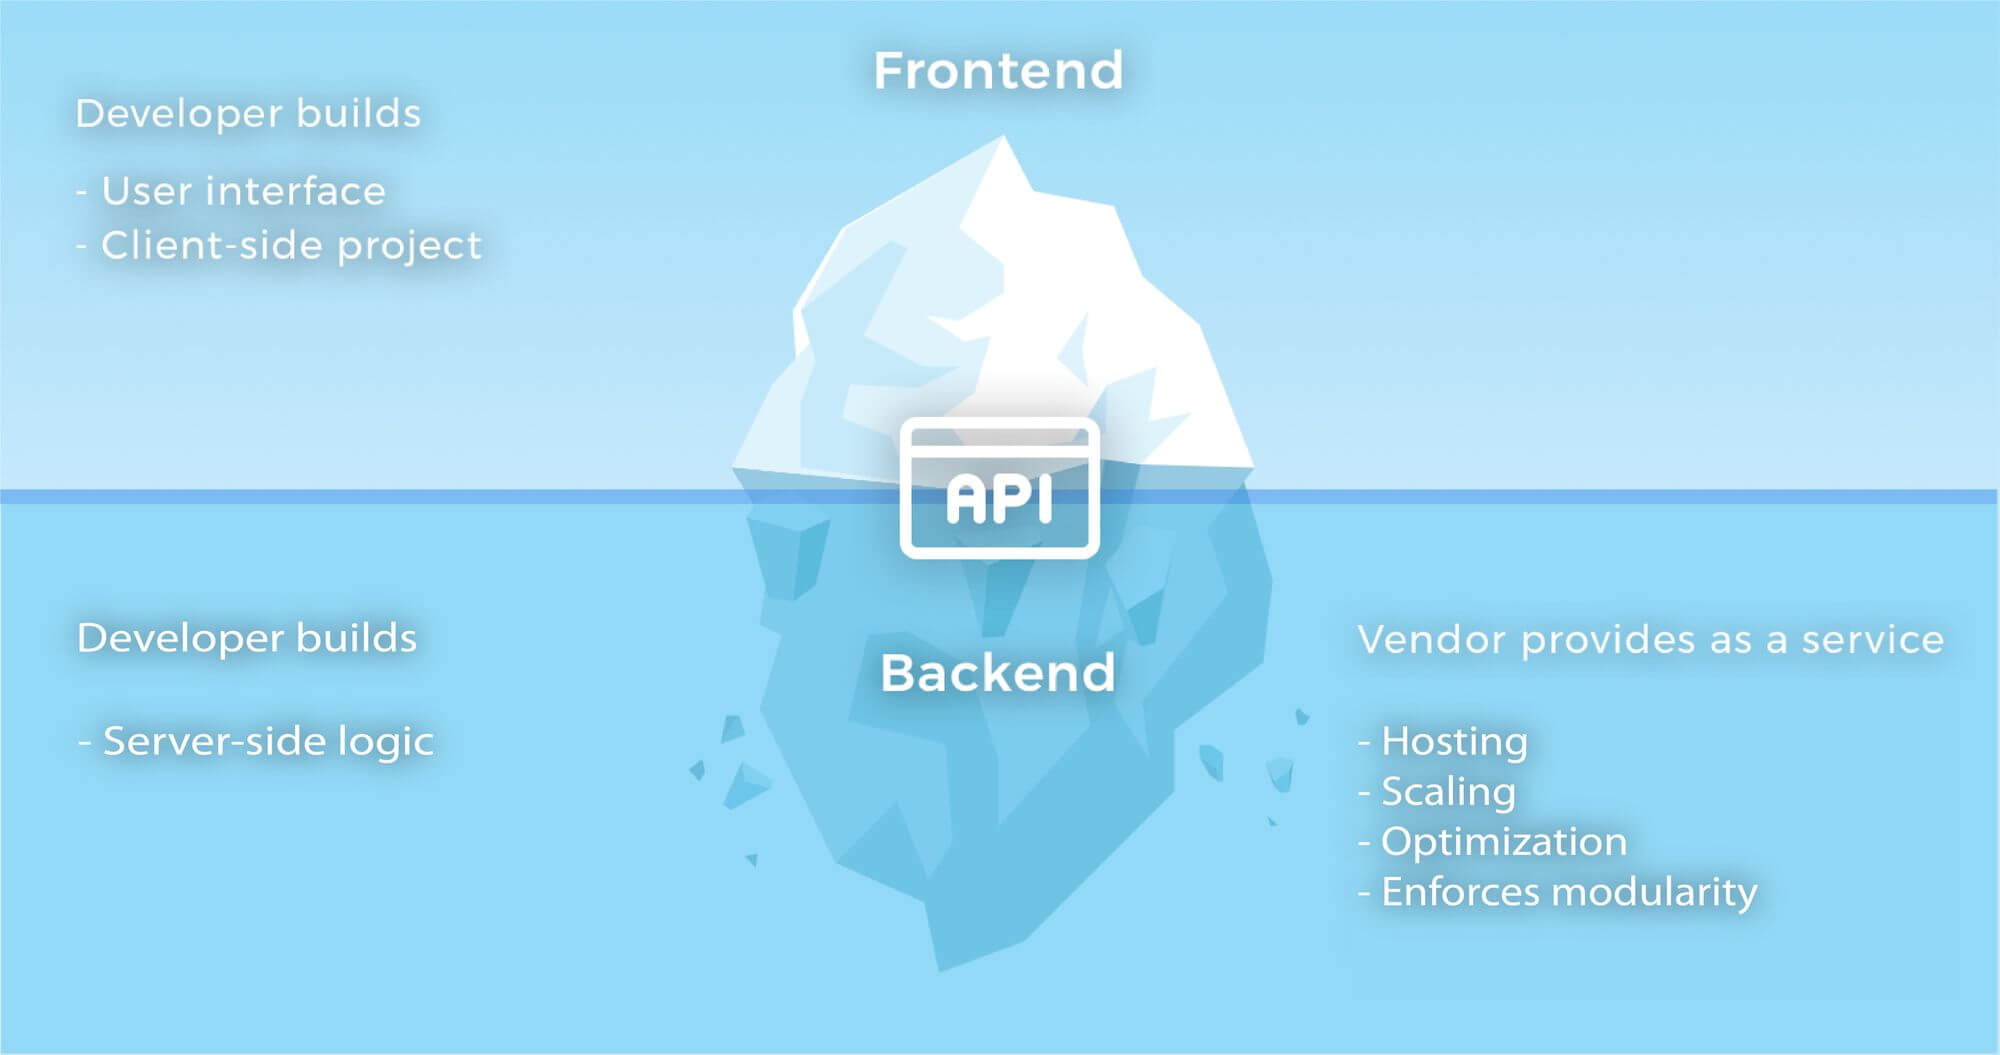
\includegraphics[width=\textwidth]{images/faas.jpg}
\end{frame}

\begin{frame}{FaaS Example}
    \begin{adjustwidth}{-12mm}{-12mm}
        \centering
        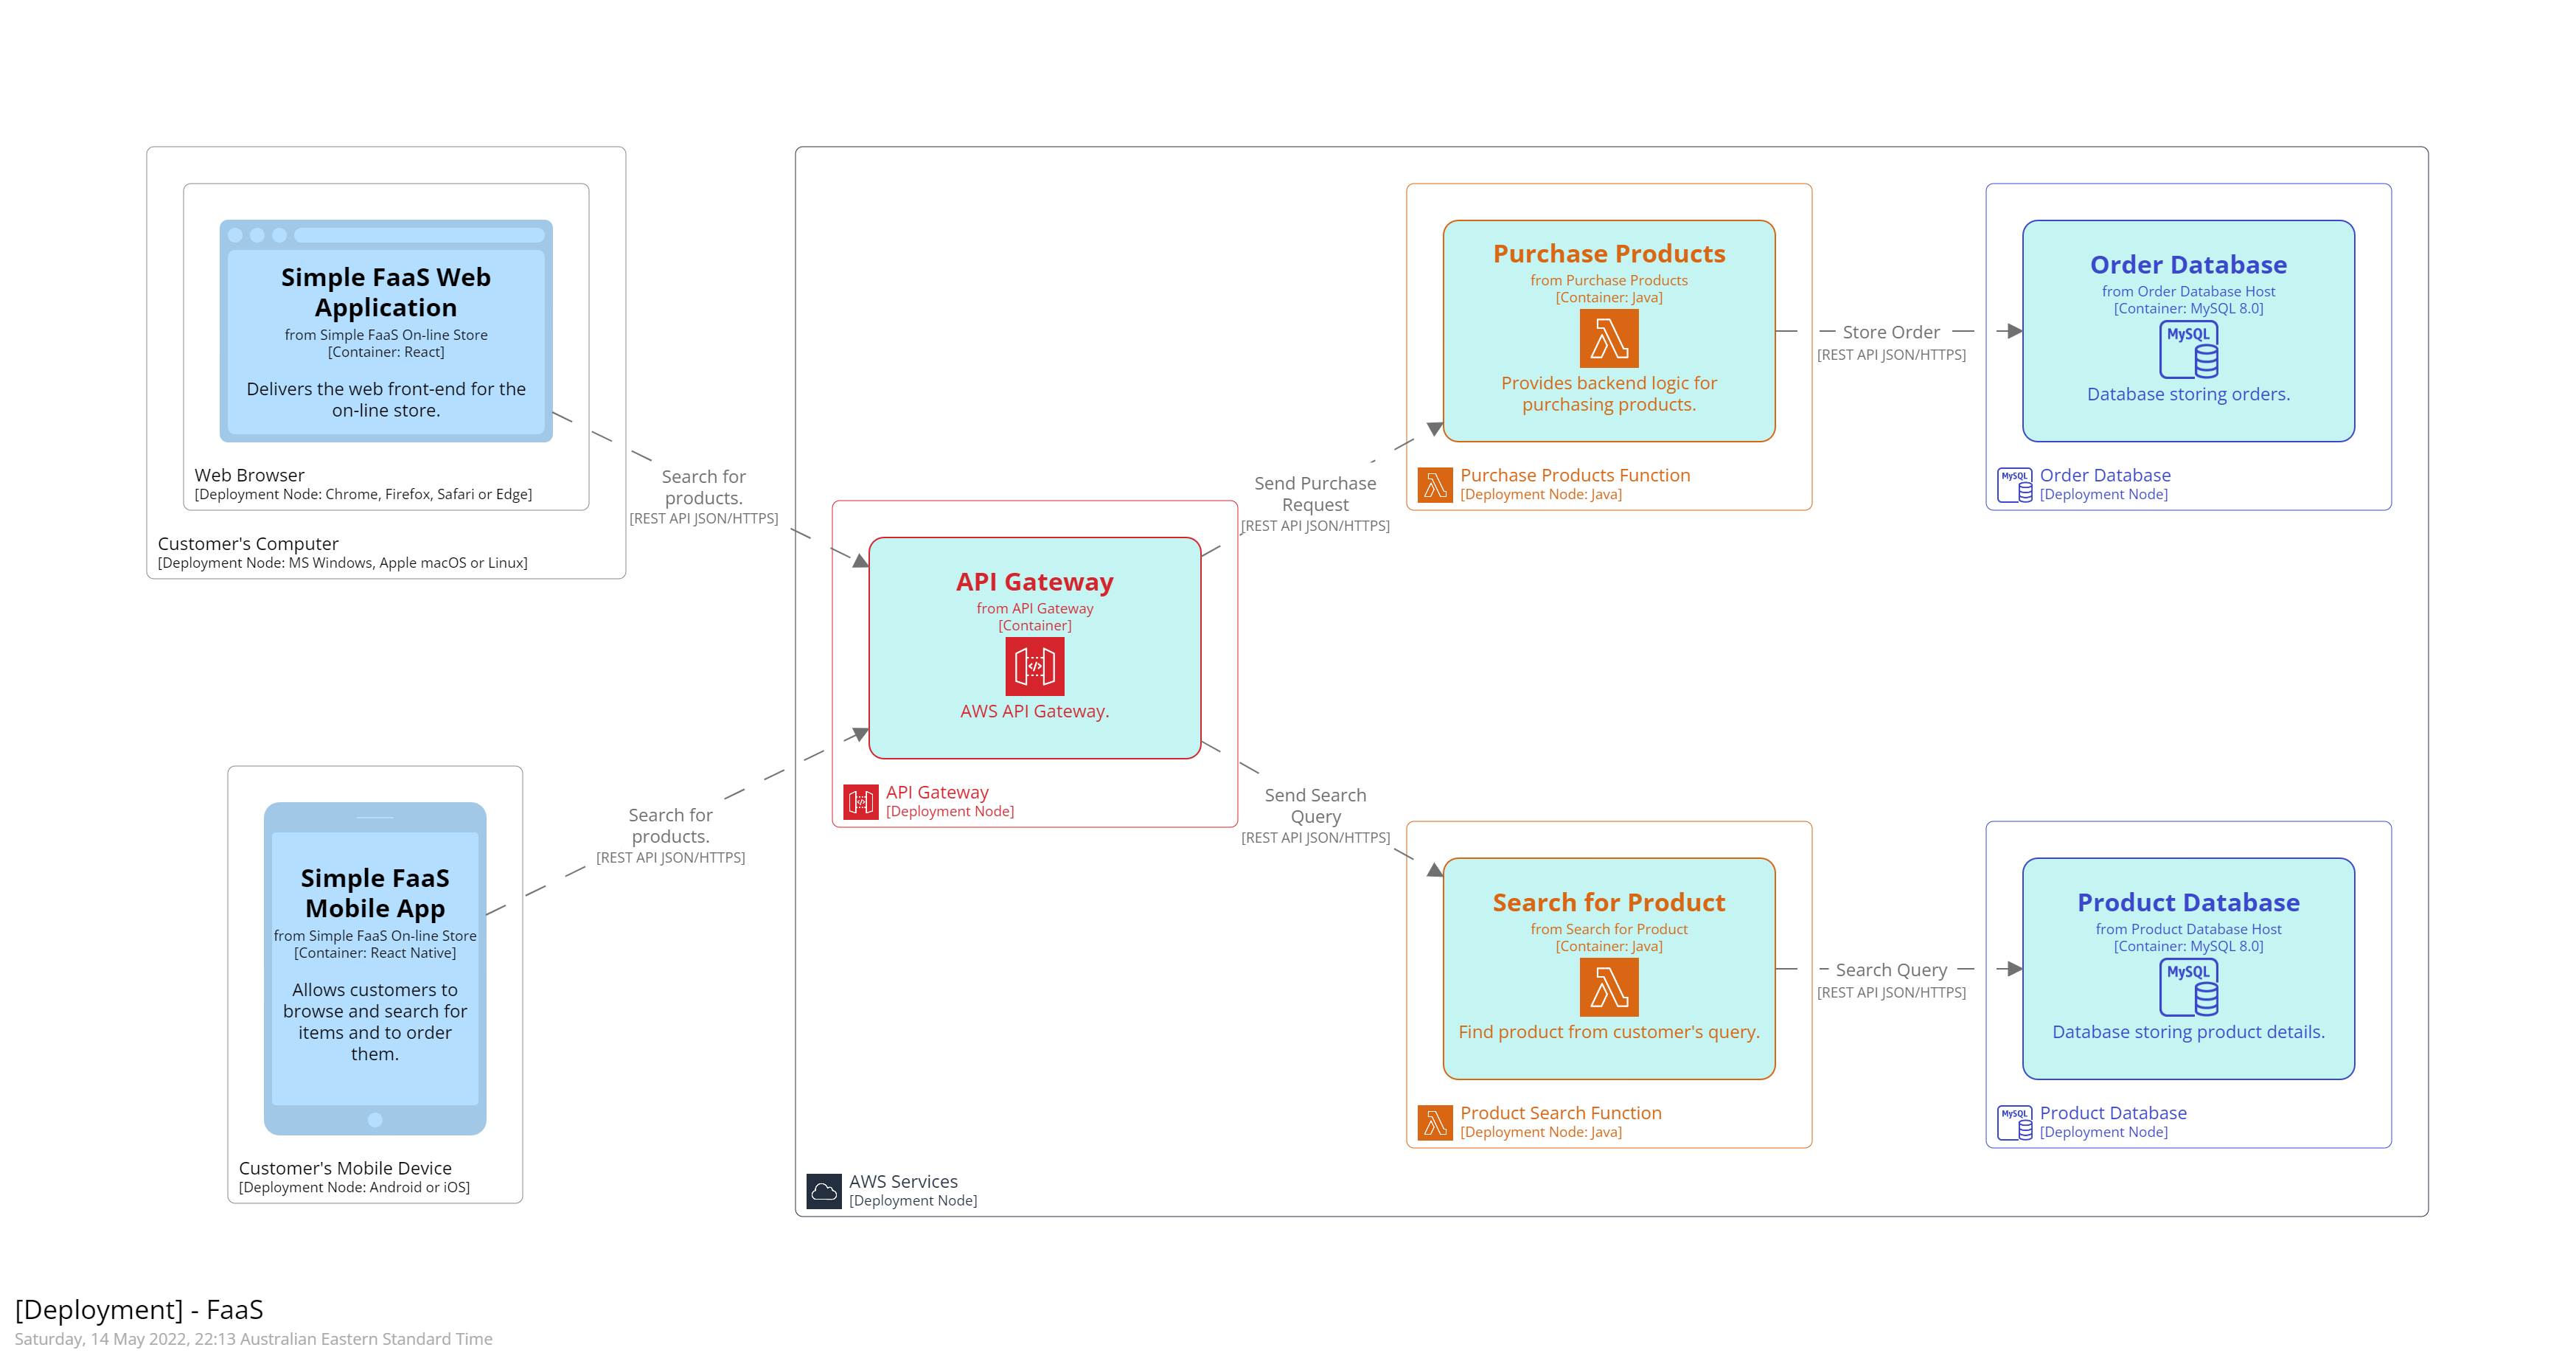
\includegraphics[trim=195 195 195 195,clip,width=0.99\paperwidth]{diagrams/faas-example.png}
    \end{adjustwidth}
\end{frame}
\note[itemize]{
    \item Example of simple system with back-end functionality delivered entirely by FaaS.
    \item Feature-rich front-ends coordinate behaviour delivered by FaaS.
    \item Front-ends invoke functions via an API.
    \item API Gateway provides some separation between front-end and functions.
    \item May allow a bit more separation between UI and logic.
}

\definition{Serverless Architecture}{Software system delivering functionality through BaaS or FaaS.}
\note[itemize]{
    \item Many people focus on FaaS when considering Serverless.
    \item Some simple Single Page Web Apps (SPA) coordinate.
    \item Front-end ties back-end services together to deliver the application's functionality.
}

\begin{frame}{Sahara Browse \& Order}
    \begin{adjustwidth}{-12mm}{-12mm}
        \centering
        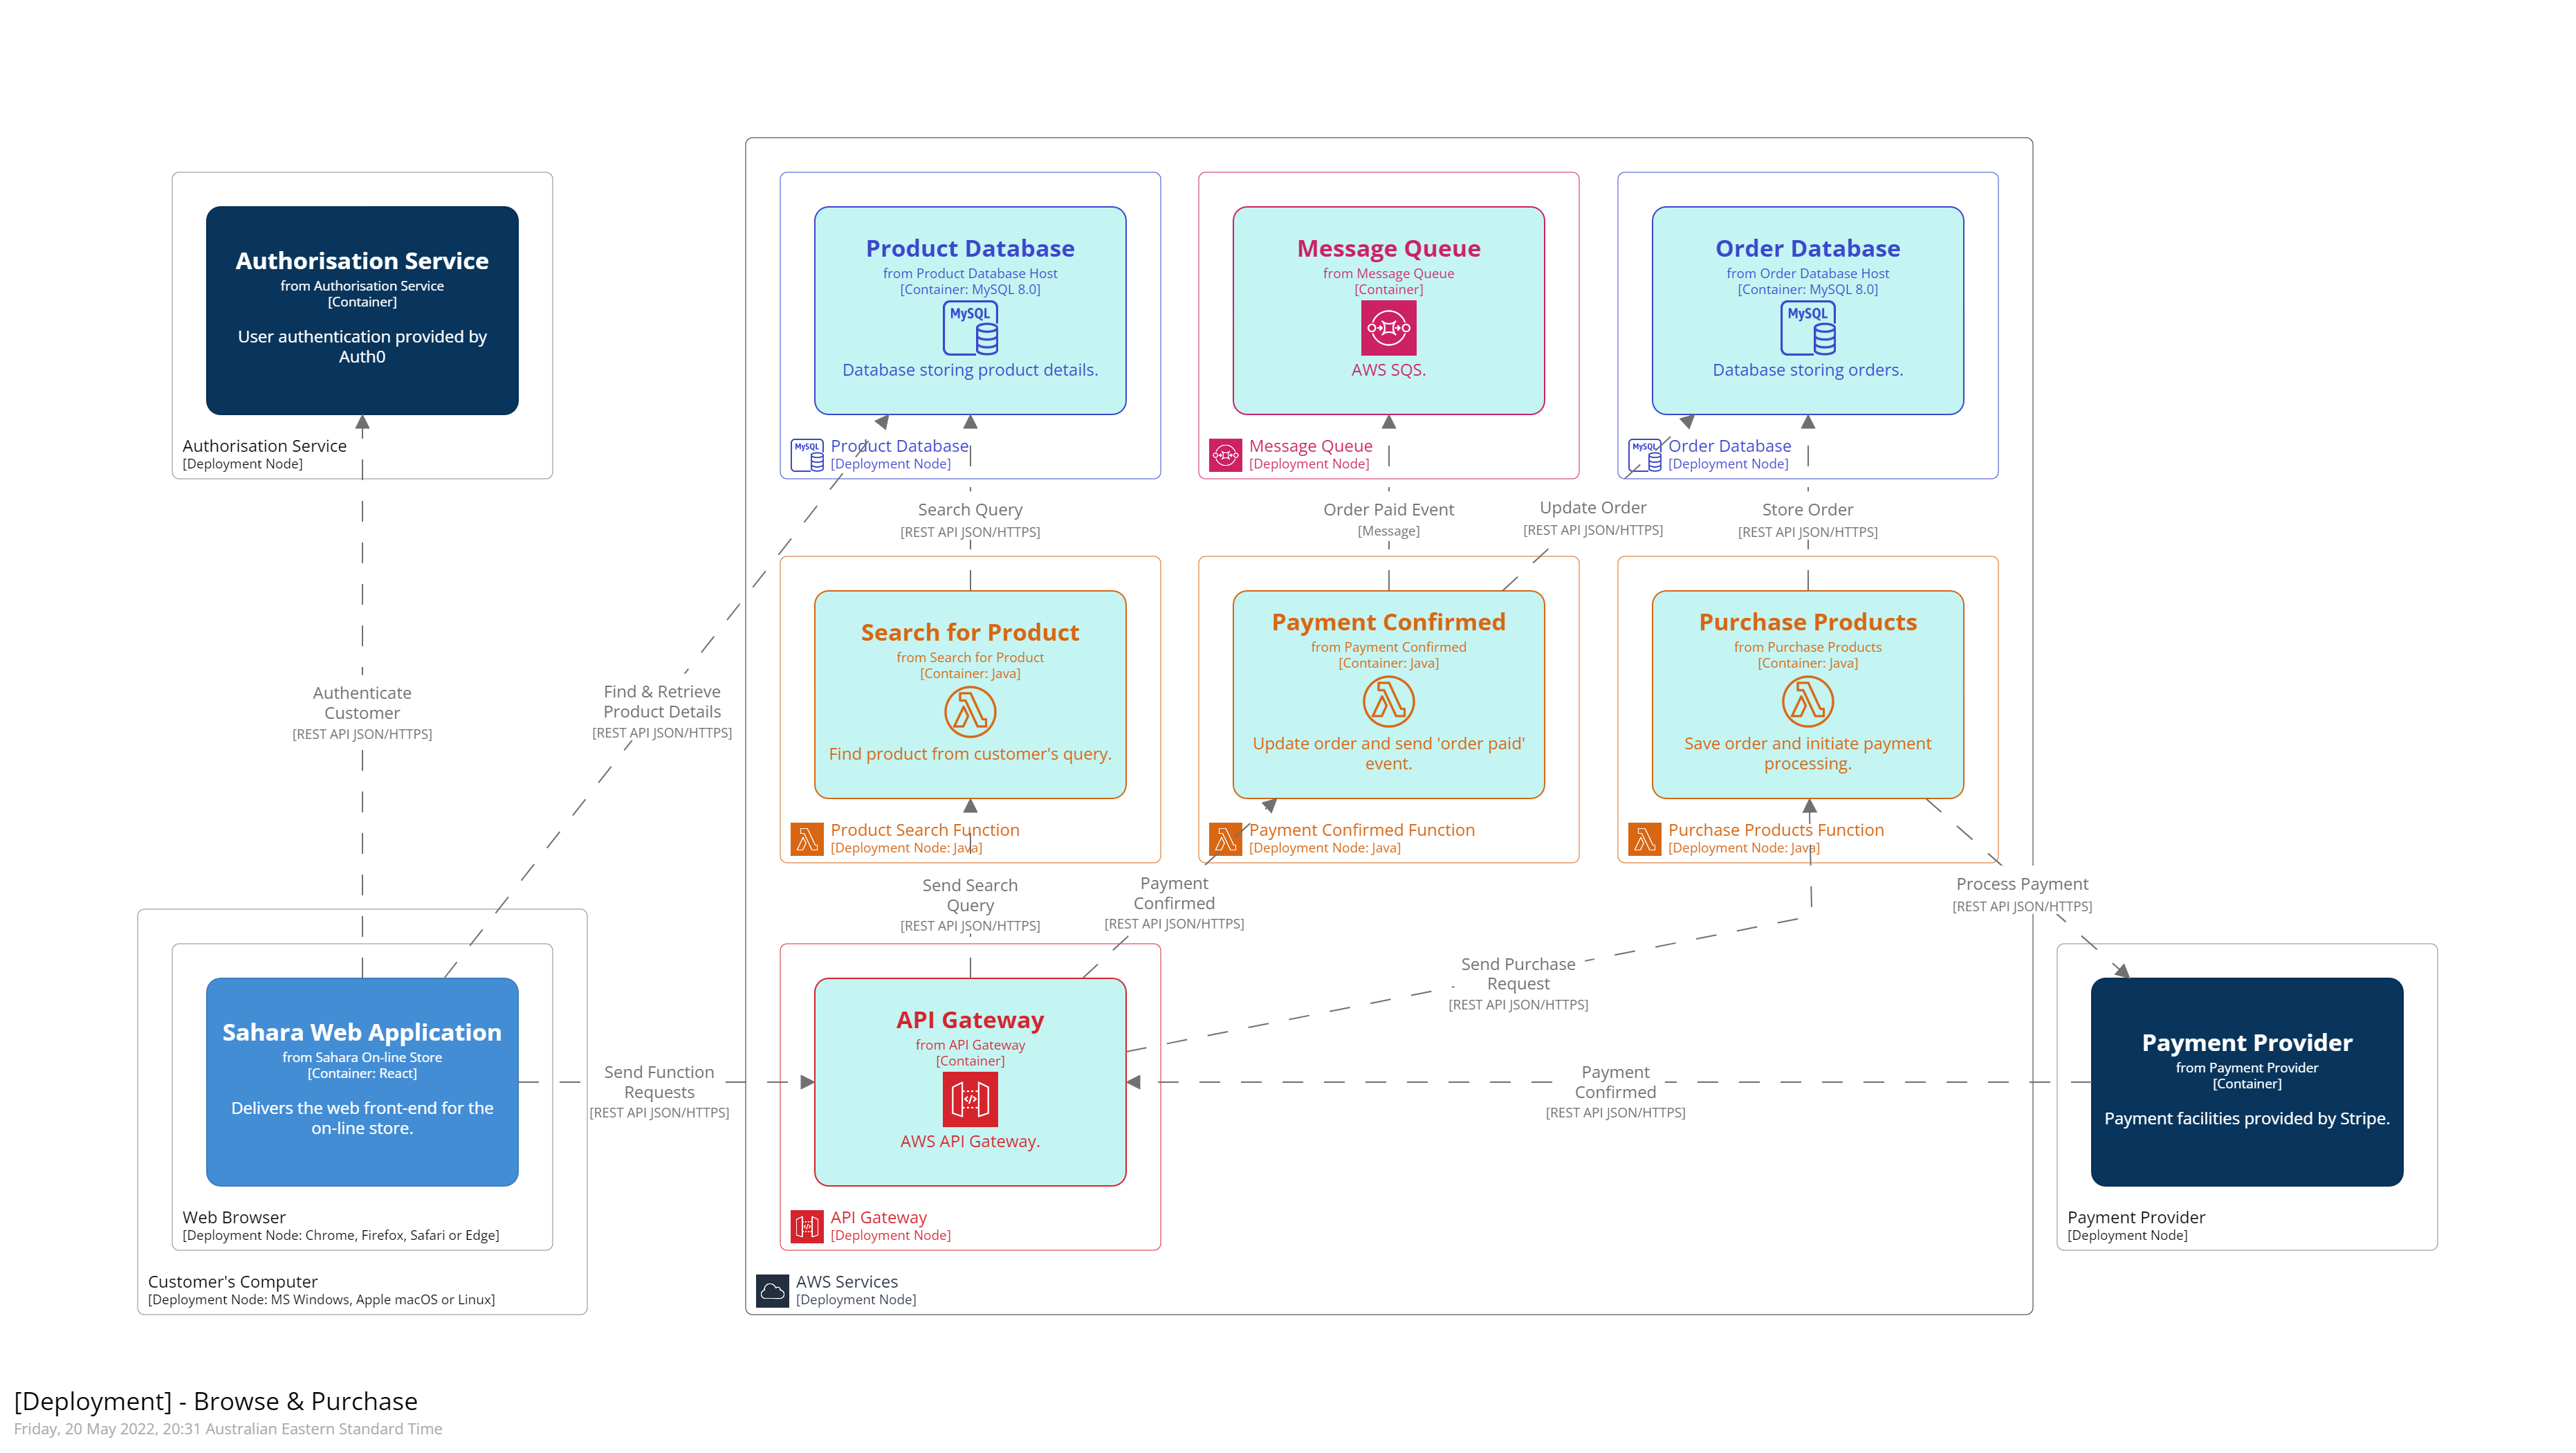
\includegraphics[trim=195 195 195 195,clip,width=0.99\paperwidth]{diagrams/sahara-deployment-1.png}
    \end{adjustwidth}
\end{frame}
\note[itemize]{
    \item Sahara eCommerce example as a serverless app.
    \item Only browse, search and purchase are shown.
    \item Point out that it uses both BaaS \& FaaS.
    \item Shopping cart is implemented within the web and mobile app for this architecture.
    \item Order Scenario 1: Customer checks out their shopping cart in the web or mobile app.
    \item Order Scenario 2: App calls Purchase Products function via API Gateway.
    \item Order Scenario 3: Purchase Products stores order in DB and sends a payment request to Payment Provider.
    \item Order Scenario 4: We provide Payment Provider with API end point to call to report payment result.
    \item Order Scenario 5: Payment success causes Payment Confirmed function to be invoked.
    \item Order Scenario 6: Payment Confirmed updates order in DB with payment status.
    \item Order Scenario 7: Payment Confirmed adds Payment Confirmation message to the Queue.
    \item Order Scenario 8: Payment Confirmation message is picked up by a fulfillment function to pack \& send order.
    \item Order Scenario 9: Once order is shipped, another message would trigger an `order sent' function.
}

\begin{frame}{Sahara Fulfilment}
    \begin{adjustwidth}{-12mm}{-12mm}
        \centering
        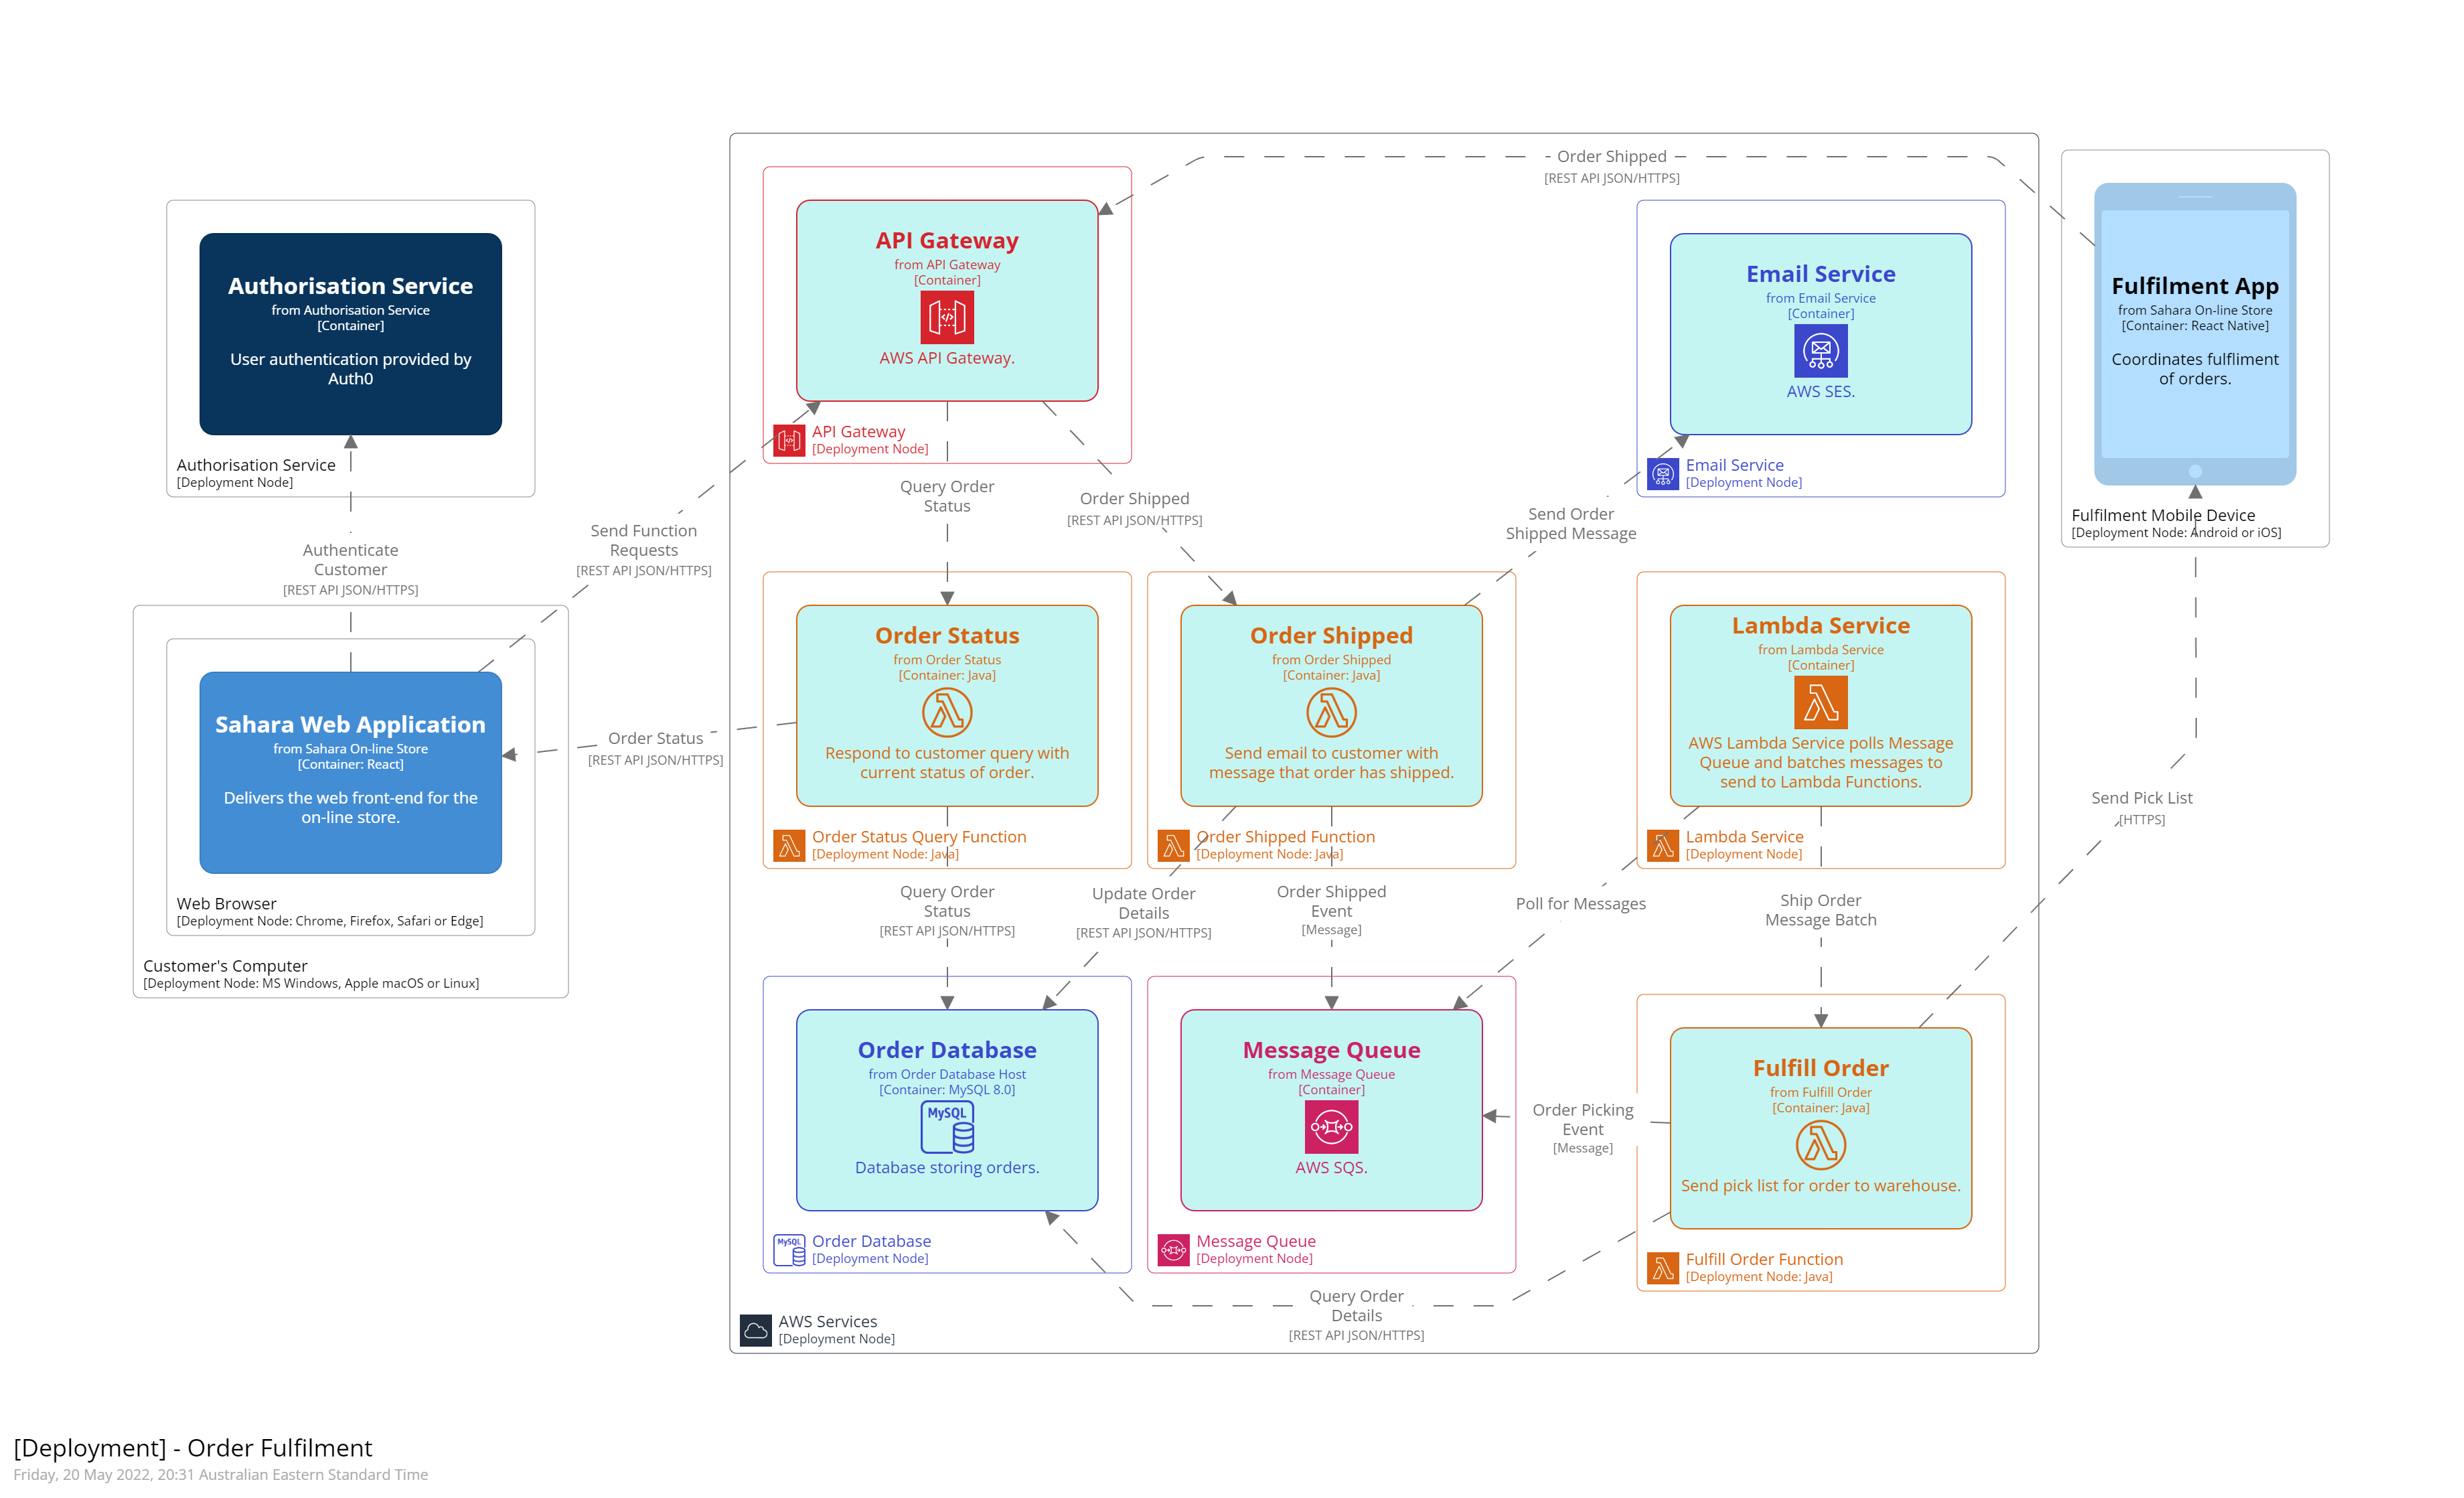
\includegraphics[trim=195 195 195 195,clip,width=0.92\paperwidth]{diagrams/sahara-deployment-2.png}
    \end{adjustwidth}
\end{frame}
\note[itemize]{
    \item Sahara eCommerce example as a serverless app.
    \item Only fulfilment functions are shown.
    \item Shows Lambda Service polling Queue, demonstrating how Lambda Functions are invoked via events in a message queue.
    \item Fulfilment Scenario 1: Lambda Service monitors Queue for `ship order' messages.
    \item Fulfilment Scenario 2: Lambda Service batches groups of `ship order' messages and sends them to Fulfill Order function.
    \item Fulfilment Scenario 3: Fulfill Order gets order details from DB and sends pick list to Fulfilment App.
    \item Fulfilment Scenario 4: When order is shipped, Fulfilment App calls Order Shipped function via API Gateway.
    \item Fulfilment Scenario 5: Order Shipped sends email to customer and updates order status in DB.
    \item Fulfilment Scenario 5a: Simplification of order picking, packing and shipping steps.
    \item Fulfilment Scenario 5b: Each step sends messages to Queue to trigger other functions.
    \item Fulfilment Scenario 6: Customer queries order status in the web or mobile app.
    \item Fulfilment Scenario 7: App calls Order Status function via API Gateway.
    \item Fulfilment Scenario 8: Order Status queries Order DB and sends status back to customer via App.
}

\begin{frame}{Serverless Benefits}
\vspace{1pt}
{\huge
\begin{itemize}
    \item<1-> Automatic scaling
    \begin{itemize}
        \LARGE\item Multiple instances of function
    \end{itemize}
    \vspace{1mm}
    \item<2-> Reduced cost for dynamic loads
    \begin{itemize}
        \LARGE\item No server idle time
    \end{itemize}
%    \vspace{1mm}
    \item<3-> Reduced server management
    \vspace{1mm}
    \item<4-> Easier to run closer to client
    \begin{itemize}
        \LARGE\item Launch in same zone as client 
    \end{itemize}
\end{itemize}
}
\end{frame}

\begin{frame}{BaaS Tradeoffs}
\vspace{1pt}
{\huge
\begin{itemize}
     \item<1-> Front-end accesses database directly
     \vspace{-2pt}
    \begin{itemize}
        \LARGE\item Front-end needs to sanitise inputs
        \vspace{2pt}
        \LARGE\item Easy to spoof messages from front-end
        \begin{itemize}
            \Large\item Hope DB provider is secure
        \end{itemize}
    \end{itemize}
    \vspace{1mm}
    \item<2-> Application logic is in front-end
    \vspace{-2pt}
    \begin{itemize}
        \LARGE\item Less modularisation
        \vspace{5pt}
        \LARGE\item Duplication of logic with multiple front-ends
        \begin{itemize}
            \Large\item Web, mobile, \dots
        \end{itemize}
    \end{itemize}
%    \vspace{2mm}
    \item<3-> No control over server optimisation
\end{itemize}
}
\end{frame}
\note[itemize]{
    \item Spoofing messages is an issue for all BaaS services.
    \item Modern expectations are that almost all systems will have multiple front-ends.
    \item Duplication of front-end logic is a smaller, but still partial, concern for FaaS.
}

\begin{frame}{FaaS Tradeoffs}
\vspace{1pt}
{\huge
\begin{itemize}
    \item<1-> No server state
    \vspace{5pt}
    \begin{itemize}
        \LARGE\item All state needs to be saved (e.g. Redis, S3, \dots)
        \begin{itemize}
            \Large\item Not just persistent state
        \end{itemize}
    \end{itemize}
    \vspace{1mm}
    \item<2-> Execution duration
    \vspace{4pt}
    \begin{itemize}
        \LARGE\item Can't be long running process
        \begin{itemize}
            \Large\item AWS Lambda is up to 15 minutes
        \end{itemize}
    \end{itemize}
    \vspace{1mm}
    \item<3-> Startup latency
    \begin{itemize}
        \LARGE\item Functions take time to start
        \begin{itemize}
            \Large\item Some languages worse than others (e.g. Java)
        \end{itemize}
    \end{itemize}
    \vspace{1mm}
    \item<4-> Proliferation of functions
    \begin{itemize}
        \LARGE\item Loss of encapsulation
    \end{itemize}
\end{itemize}
}
\end{frame}
\note[itemize]{
    \item Server running function can be killed when function is not running.
    \item Can occassionally send messages to functions to keep them alive.
    \item Java has concurrency benefits over other languages.
}

\questionanswer{When is serverless appropriate?}{
    \begin{itemize}
        \item<2-> Rich client apps with common backend
            \begin{itemize}
                \Large\item BaaS
            \end{itemize}
        \vspace{1mm}
        \item<3-> High latency processing
            \begin{itemize}
                \Large\item Within function duration constraints
            \end{itemize}
        \vspace{1mm}
        \item<4-> Apps with variable load
            \begin{itemize}
                \Large\item Take advantage of auto-scaling
            \end{itemize}
    \end{itemize}
}

\questionanswer{When is serverless \highlight{not} appropriate?}{
    \begin{itemize}
        \item<2-> Quick response required
            \begin{itemize}
                \Large\item Can't wait for FaaS to start
            \end{itemize}
        \item<3-> Compute intensive processing
        \vspace{1mm}
        \item<4-> Apps with steady load
            \begin{itemize}
                \Large\item Server-based approaches are cheaper
            \end{itemize}
    \end{itemize}
}

\point[Self-Study Exercise]{
\begin{itemize}
    \item Redesign your scalability assignment to be serverless.
     \begin{itemize}
        \LARGE\item What parts of your design would benefit from being serverless?
    \end{itemize}
   \vspace{2mm}
    \item Implement your revised design.
\end{itemize}
}

\begin{frame}{Pros \& Cons}
    \vspace{1mm}
    {\LARGE
    \begin{description}
        \item[Extensibility] \tabto{15em}
\includegraphics[width=8mm]{../../shared/images/thumbs-up.png}
        \item[Reliability] \tabto{15em}
\includegraphics[width=8mm]{../../shared/images/thumbs-up.png}
        \item[Interoperability] \tabto{15em}
\includegraphics[width=8mm]{../../shared/images/thumbs-up.png}
        \item[Scalability] \tabto{15em}
\includegraphics[width=8mm]{../../shared/images/thumbs-up.png}
        \item[Deployability] \tabto{15em}
\includegraphics[width=8mm]{../../shared/images/thumbs-up.png}
        \item[Modularity] \tabto{15em}
\includegraphics[width=8mm]{../../shared/images/neutral.png}
        \item[Testability] \tabto{15em}
\includegraphics[trim=22 19 22 12,clip,width=8mm]{../../shared/images/neutral.png}
        \item[Security] \tabto{15em}
\includegraphics[trim=22 19 22 12,clip,width=8mm]{../../shared/images/thumbs-down.png}
        \item[Simplicity] \tabto{15em}
\includegraphics[trim=22 19 22 12,clip,width=8mm]{../../shared/images/thumbs-down.png}
    \end{description}
    }
\end{frame}
\note[itemize]{
    \item Modularity: Deployed functions are naturally modular.
    \item Modularity: Higher-level abstractions to group deployed functions is difficult.
    \item Testability: Unit testing FaaS functions is easy.
    \item Testability: Integration testing is hard.
    \item Security BaaS: Front-end access database directly. No server-side protection of db.
    \item Security FaaS: Every function needs its own security policy (e.g. IAM), which is easy to get wrong.
}

\references{serverless}

\end{document}